\section{System description}
The ray tracing engine will be divided into 3 parts :
\begin{itemize}
  \item XML parser
  \item World objects
  \item Engine
\end{itemize}

The xml parser have an xml file as input. This xml must describe the scene which will be rendered. The syntax for this xml will be describe in the analysis phase and will be handed with a XML Scheme descriptor. This parser will produce the World object.

The world objects are all the object which can be used to describe a scene. The exhaustive list of these objects are :
\begin{itemize}
  \item Sphere
  \item Cube
  \item Cylinder
\end{itemize}

We can also do transformations on these objects : rotation, translation, scaling.

Finally, the engine will render an image using the world objects.

\begin{figure}[ht]
  \centering
  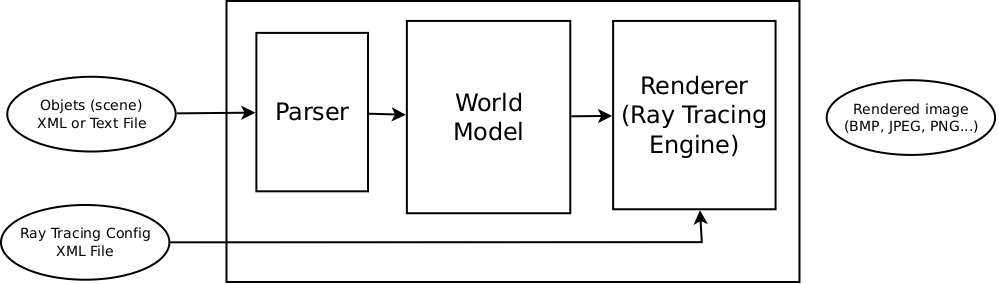
\includegraphics[height=5cm]{img/modules.png}
  \caption{Modules}
  \label{modules}
\end{figure}

